\begin{frame}{MiniZinc: Group Photo}
\textbf{Exercise 3}

Given a group of $n$ people, we must arrange them for a photo. The best
photo is when people are next to their friends, so the aim is to arrange them so that each person
is next to (to the left or right) with as many friends as possible. The data for the
problem is given as
%
\begin{align*}
& \texttt{n = <size of problem> ;} \\
& \texttt{array[1..n,1..n] of var bool: friend; }
\end{align*} 
%
where \texttt{friend[f1, f2]} means \texttt{f1} and \texttt{f2} are friends. You can assume that the friend array is symmetric.
You should output a list of the people in their position to maximize the number of adjacent
friends. For example given the data \texttt{groupphoto1.dzn}, you should output the placement of the guests as well as the objective value, i.e.,

\begin{align*}
& \texttt{Obj = 7; [4, 3, 5, 6, 8, 7, 1, 2]}
\end{align*}


\begin{textblock*}{4cm}[1,1](\textwidth,\textheight-0.33cm)
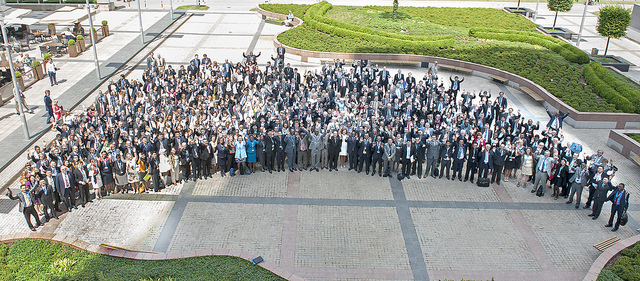
\includegraphics[width=\textwidth]{img/group-photo.jpg}
\end{textblock*}

\end{frame}
